\documentclass[10pt]{beamer}\usepackage[]{graphicx}\usepackage[]{color}
% maxwidth is the original width if it is less than linewidth
% otherwise use linewidth (to make sure the graphics do not exceed the margin)
\makeatletter
\def\maxwidth{ %
  \ifdim\Gin@nat@width>\linewidth
    \linewidth
  \else
    \Gin@nat@width
  \fi
}
\makeatother

\definecolor{fgcolor}{rgb}{0.345, 0.345, 0.345}
\newcommand{\hlnum}[1]{\textcolor[rgb]{0.686,0.059,0.569}{#1}}%
\newcommand{\hlstr}[1]{\textcolor[rgb]{0.192,0.494,0.8}{#1}}%
\newcommand{\hlcom}[1]{\textcolor[rgb]{0.678,0.584,0.686}{\textit{#1}}}%
\newcommand{\hlopt}[1]{\textcolor[rgb]{0,0,0}{#1}}%
\newcommand{\hlstd}[1]{\textcolor[rgb]{0.345,0.345,0.345}{#1}}%
\newcommand{\hlkwa}[1]{\textcolor[rgb]{0.161,0.373,0.58}{\textbf{#1}}}%
\newcommand{\hlkwb}[1]{\textcolor[rgb]{0.69,0.353,0.396}{#1}}%
\newcommand{\hlkwc}[1]{\textcolor[rgb]{0.333,0.667,0.333}{#1}}%
\newcommand{\hlkwd}[1]{\textcolor[rgb]{0.737,0.353,0.396}{\textbf{#1}}}%
\let\hlipl\hlkwb

\usepackage{framed}
\makeatletter
\newenvironment{kframe}{%
 \def\at@end@of@kframe{}%
 \ifinner\ifhmode%
  \def\at@end@of@kframe{\end{minipage}}%
  \begin{minipage}{\columnwidth}%
 \fi\fi%
 \def\FrameCommand##1{\hskip\@totalleftmargin \hskip-\fboxsep
 \colorbox{shadecolor}{##1}\hskip-\fboxsep
     % There is no \\@totalrightmargin, so:
     \hskip-\linewidth \hskip-\@totalleftmargin \hskip\columnwidth}%
 \MakeFramed {\advance\hsize-\width
   \@totalleftmargin\z@ \linewidth\hsize
   \@setminipage}}%
 {\par\unskip\endMakeFramed%
 \at@end@of@kframe}
\makeatother

\definecolor{shadecolor}{rgb}{.97, .97, .97}
\definecolor{messagecolor}{rgb}{0, 0, 0}
\definecolor{warningcolor}{rgb}{1, 0, 1}
\definecolor{errorcolor}{rgb}{1, 0, 0}
\newenvironment{knitrout}{}{} % an empty environment to be redefined in TeX

\usepackage{alltt}


%\input{slides_header.tex}
\input{/home/sahir/git_repositories/EPIB607/slides/slides_header2.tex}
\graphicspath{{/home/sahir/git_repositories/EPIB607/slides/figure/}}

%\let\oldShaded\Shaded
%\let\endoldShaded\endShaded
%\renewenvironment{Shaded}{\footnotesize\oldShaded}{\endoldShaded}

\newcommand{\blue}[1]{\textcolor{blue}{#1}}
\newcommand{\red}[1]{\textcolor{red}{#1}}


\usepackage{xparse}
\NewDocumentCommand\mylist{>{\SplitList{;}}m}
{
	\begin{itemize}
		\ProcessList{#1}{ \insertitem }
	\end{itemize}
}
\NewDocumentCommand\mynum{>{\SplitList{;}}m}
{
	\begin{enumerate}
		\ProcessList{#1}{ \insertitem }
	\end{enumerate}
}
\newcommand\insertitem[1]{\item #1}

\newcommand\FrameText[1]{%
	\begin{textblock*}{\paperwidth}(0pt,\textheight)
		\raggedright #1\hspace{.5em}
\end{textblock*}}
\IfFileExists{upquote.sty}{\usepackage{upquote}}{}
\begin{document}

	

%\title{Introduction to Regression Trees}
%\author{Sahir Bhatnagar \inst{1}}
%\author[shortname]{Sahir Rai Bhatnagar, PhD Candidate (Biostatistics) }
%\institute[shortinst]{Department of Epidemiology, Biostatistics and Occupational Health}

	\title{015 - Midterm Review}
\author{EPIB 607 - FALL 2020}
\institute{
	Sahir Rai Bhatnagar\\
	Department of Epidemiology, Biostatistics, and Occupational Health\\
	McGill University\\
	
	\vspace{0.1 in}
	
	\texttt{sahir.bhatnagar@mcgill.ca}\\
	%\texttt{\url{https://sahirbhatnagar.com/EPIB607/}}
}

\date{slides compiled on \today}

\maketitle



%\begin{frame}[label=toc]{Table of Contents}
%	\tableofcontents
%\end{frame}

%\AddButton

\section{Exam Details}
\begin{frame}{Exam Details}
	
	\begin{itemize}
		\setlength\itemsep{.51em}
		\item \textbf{When:} Friday October 23, 3:35pm - 5:35pm.
		\item This is a 2 hour, open book exam. Any material on myCourses (EPIB607/613) and personal notes are permitted.
		\item You are not permitted to use the internet and you must work alone. Using the internet or obtaining help from anyone else is considered Cheating as per \href{https://www.mcgill.ca/students/srr/academicrights/integrity/cheating}{Article 17 of the Code of Student Conduct and Disciplinary Procedures}
%	\item The exam is out of 70. There are 7 questions, each worth 10 points. Write down all your answers in the provided booklet. 
		\item Provide units and state your assumptions when applicable. Label axes and write answers in complete sentences when appropriate.
		\item The format of the exam will follow the assignments. That is, you will be required to complete a series of questions in an RMarkdown document and knit to pdf. Your solutions for each question must then be uploaded to Crowdmark. A template will be provided.
		\item You will be given 1 extra hour to upload your solutions.
		%\item Some commonly used $z$ and $t$ quantiles will be provided in a Table. If a question requires the use of $z$ or $t$ probabilites/quantiles not found in the provided Table, write the corresponding R code instead. When possible, you should complete the calculations.
		
	\end{itemize}
	
\end{frame}

\begin{frame}{Topics to be covered}
	
	\begin{enumerate}
		\setlength\itemsep{.51em}
		\item Data visualization (histograms, boxplots, scatterplots, line plots), Tidy Data, Color Palettes
		\item Descriptive statistics (mean, median, range, IQR, sd, correlation)
		\item Normal Curve Calculations
		\item Sampling Distributions, CLT, Bootstrap
		\item Confidence intervals and p-values for one sample mean and one sample proportion
		\item Hypothesis Testing
		\item Power and Sample size calculations
	\end{enumerate}
	
\end{frame}

\section{Data visualization}

\begin{frame}{Aesthetics}
	\begin{itemize}
		\setlength\itemsep{.51em}
		\item Aesthetics
		\framedgraphic{scales.jpg}
		\pause 
		\item Commonly used aesthetics in data visualization: position, shape, size, color, line width, line type. Some of these aesthetics can represent both continuous and discrete data (position, size, line width, color) while others can only represent discrete data (shape, line type)	
	\end{itemize}
\end{frame}

\begin{frame}{Types of Graphs}
	\begin{itemize}
		\item Review the types of graphs created in the assignments.
		\item You should be able to critique a graph and propose appropriate graphics for a given dataset. Be mindful of the research question. The graphic should try to answer the research question. 
		\item \url{https://serialmentor.com/dataviz/directory-of-visualizations.html}
		\item \url{https://www.data-to-viz.com/}
	\end{itemize}
\end{frame}


\begin{frame}[fragile]{Boxplots with qualitative palette}
\begin{knitrout}\tiny
\definecolor{shadecolor}{rgb}{0.969, 0.969, 0.969}\color{fgcolor}\begin{kframe}
\begin{alltt}
\hlkwd{library}\hlstd{(oibiostat);} \hlkwd{data}\hlstd{(}\hlstr{"famuss"}\hlstd{)}
\hlkwd{library}\hlstd{(ggplot2)}
\hlkwd{library}\hlstd{(colorspace)}

\hlkwd{ggplot}\hlstd{(famuss,} \hlkwd{aes}\hlstd{(}\hlkwc{x} \hlstd{= actn3.r577x,} \hlkwc{y} \hlstd{= bmi,} \hlkwc{fill} \hlstd{= actn3.r577x))} \hlopt{+}
\hlkwd{geom_boxplot}\hlstd{()} \hlopt{+}
\hlstd{colorspace}\hlopt{::}\hlkwd{scale_fill_discrete_qualitative}\hlstd{()}
\end{alltt}
\end{kframe}

{\centering 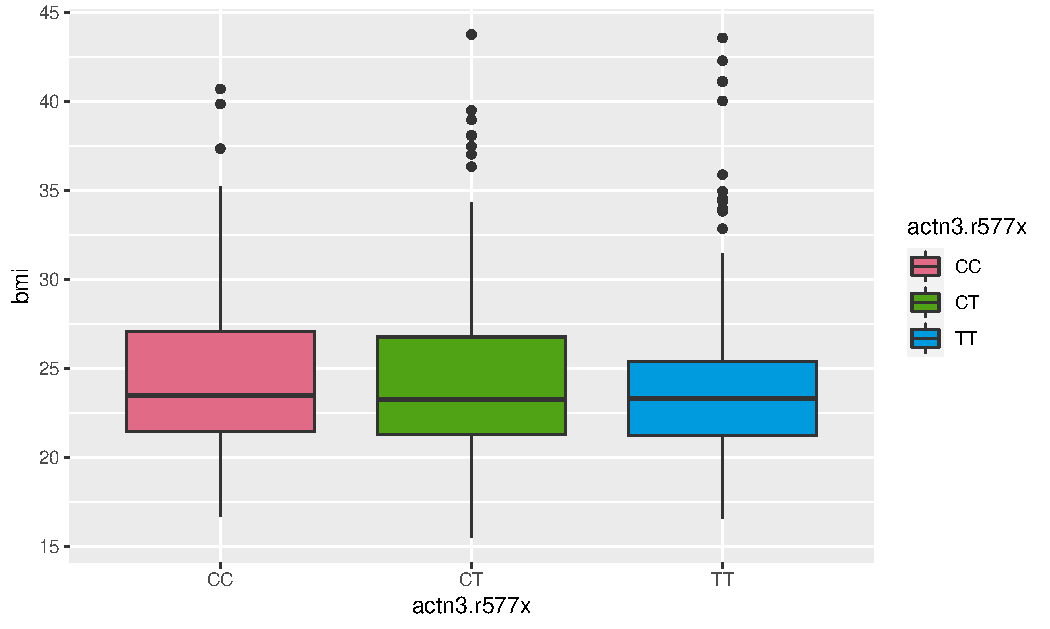
\includegraphics[width=\maxwidth]{figure/unnamed-chunk-1-1} 

}



\end{knitrout}
\end{frame}


\begin{frame}[fragile]{Conditional distribution of genotype \textit{given} race}
\begin{knitrout}\tiny
\definecolor{shadecolor}{rgb}{0.969, 0.969, 0.969}\color{fgcolor}\begin{kframe}
\begin{alltt}
\hlstd{sjPlot}\hlopt{::}\hlkwd{plot_xtab}\hlstd{(famuss}\hlopt{$}\hlstd{race, famuss}\hlopt{$}\hlstd{actn3.r577x,} \hlkwc{margin} \hlstd{=} \hlstr{"row"}\hlstd{)}
\end{alltt}
\end{kframe}

{\centering 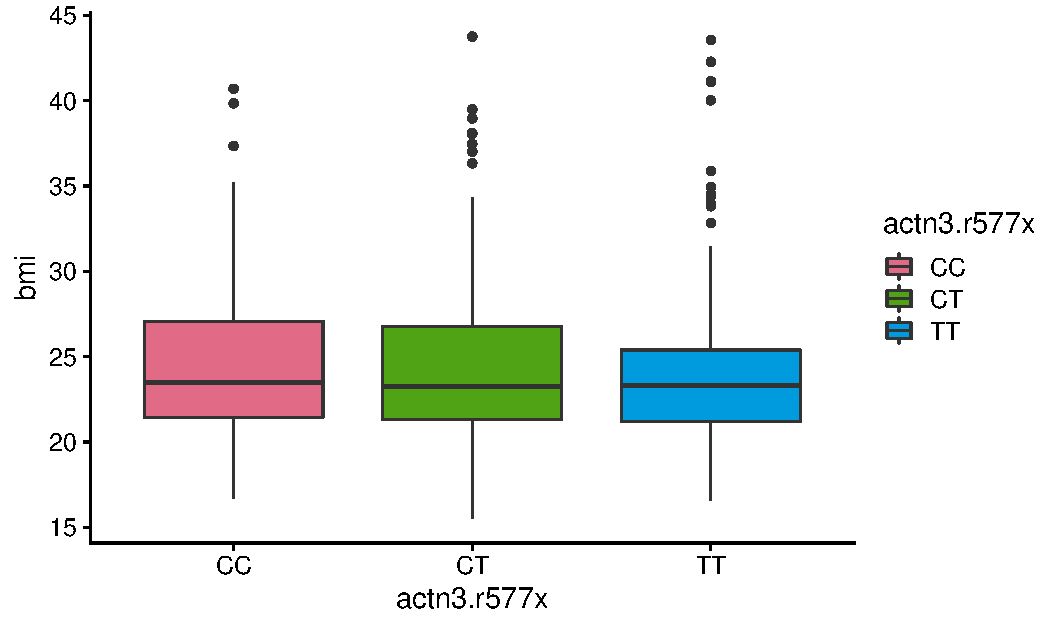
\includegraphics[width=\maxwidth]{figure/unnamed-chunk-2-1} 

}



\end{knitrout}
\end{frame}





	\begin{frame}[fragile]{Scatter plots with sequential palette}
\begin{knitrout}\tiny
\definecolor{shadecolor}{rgb}{0.969, 0.969, 0.969}\color{fgcolor}\begin{kframe}
\begin{alltt}
\hlkwd{ggplot}\hlstd{(famuss,} \hlkwd{aes}\hlstd{(}\hlkwc{x} \hlstd{= height,} \hlkwc{y} \hlstd{= weight,} \hlkwc{color} \hlstd{= bmi))} \hlopt{+}
\hlkwd{geom_point}\hlstd{()} \hlopt{+}
\hlstd{colorspace}\hlopt{::}\hlkwd{scale_color_continuous_sequential}\hlstd{(}\hlkwc{palette} \hlstd{=} \hlstr{"Viridis"}\hlstd{)}
\end{alltt}
\end{kframe}

{\centering 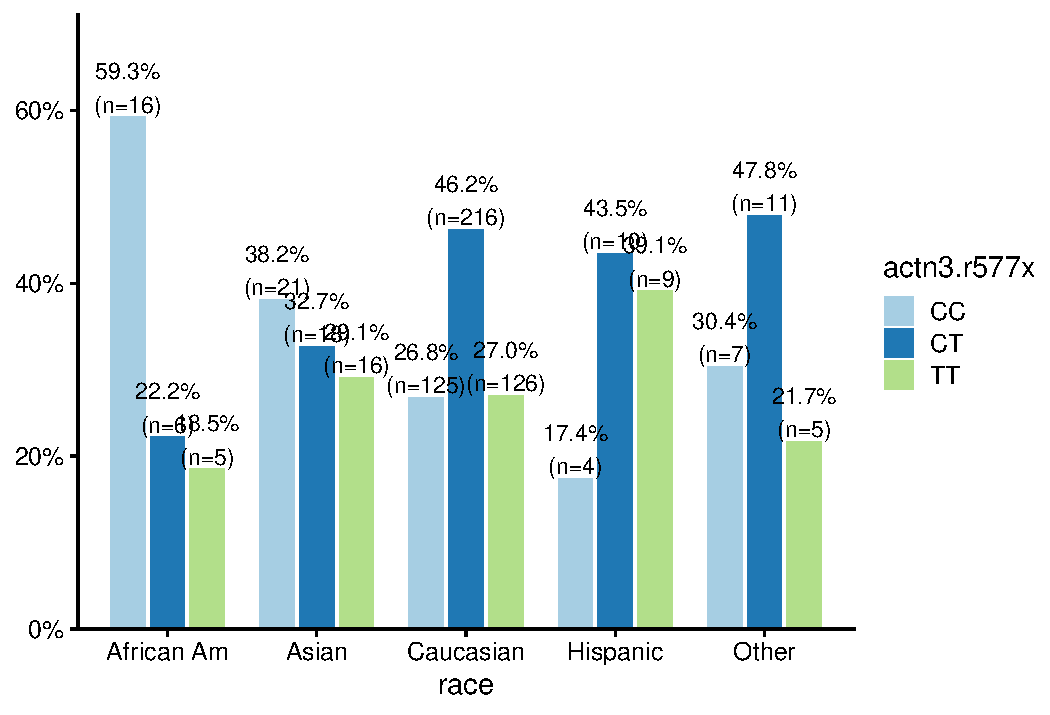
\includegraphics[width=\maxwidth]{figure/unnamed-chunk-3-1} 

}



\end{knitrout}
\end{frame}



\begin{frame}{Variable Types}
	\begin{itemize}
		\setlength\itemsep{1.5em}
		\item quantitative/numerical continuous (1.3, 5.7, 83, $1.5\times 10^{-2}$)
		\item quantitative/numerical discrete (1,2,3,4)
		\item qualitative/categorical unordered (dog, cat, fish)
		\item qualitative/categorical ordered (good, fair, poor)
	\end{itemize}
	
	
	
\end{frame}




\begin{frame}[fragile]{Color Palettes: Cynthia Brewer}
	
\begin{knitrout}\tiny
\definecolor{shadecolor}{rgb}{0.969, 0.969, 0.969}\color{fgcolor}\begin{kframe}
\begin{alltt}
\hlstd{pacman}\hlopt{::}\hlkwd{p_load}\hlstd{(RColorBrewer)}
\hlstd{RColorBrewer}\hlopt{::}\hlkwd{display.brewer.all}\hlstd{()}
\end{alltt}
\end{kframe}

{\centering 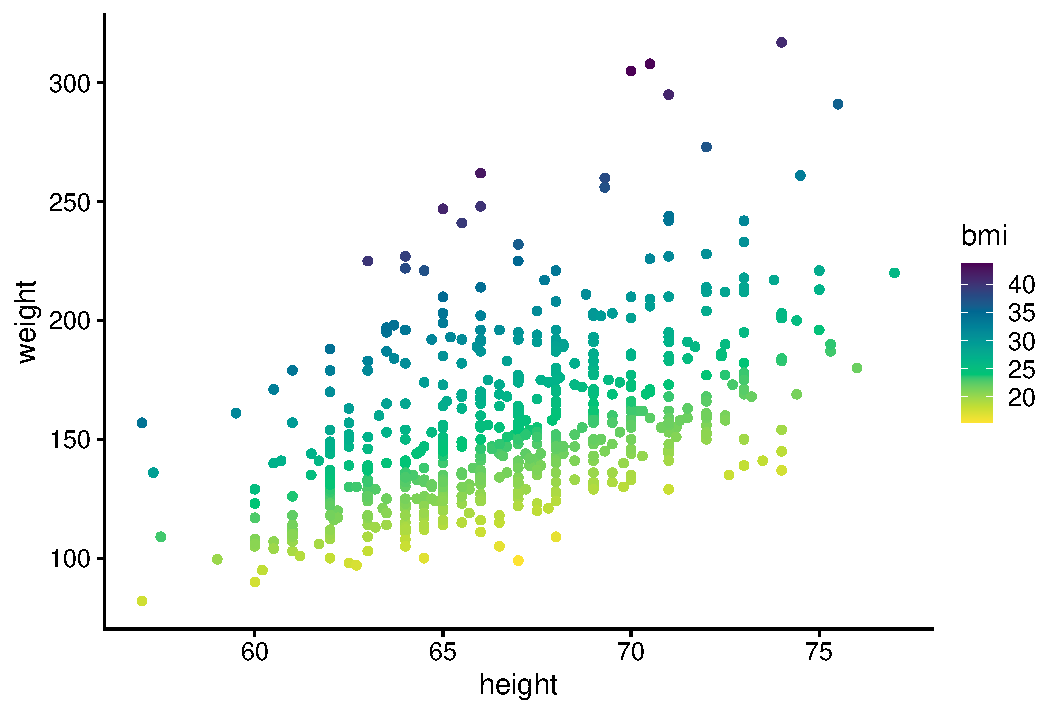
\includegraphics[width=\maxwidth]{figure/unnamed-chunk-4-1} 

}



\end{knitrout}
	
	
\end{frame}



\begin{frame}[fragile]{Color Palettes: viridis}
	
	
	
	\framedgraphic{viridis.png}
	
	
\end{frame}

\section{Tidy Data}

\begin{frame}{Tidy data}
	
	\begin{itemize}
		\setlength\itemsep{.51em}
		\item Each variable forms a column.
		\item Each observation forms a row.
		\item Each type of observational units forms a table
		\item Tidy data is ready for regression routines and plotting
	\end{itemize}
	
	
	\framedgraphic{tidy.png}
	
\end{frame}




\begin{frame}[fragile]{Example: Is it tidy?}
	
	\centering
	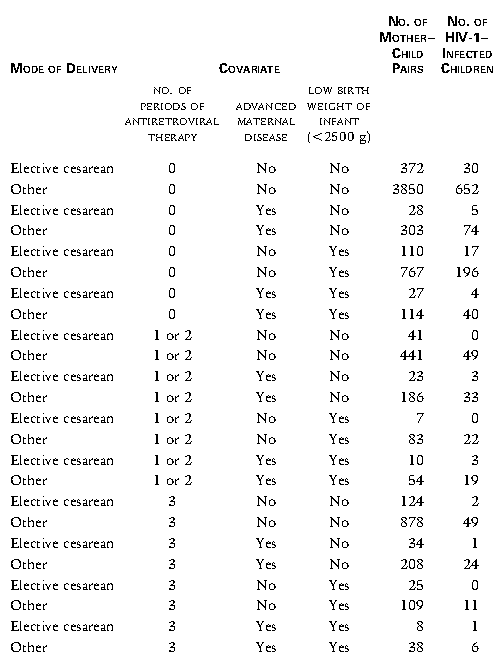
\includegraphics[scale=0.8]{hivtable.pdf}
	
	
\end{frame}

\section{Descriptive statistics}


\begin{frame}{Descriptive statistics}
	\begin{itemize}
		\setlength\itemsep{1.5em}
		\item Boxplots, histograms, density plot
		\item IQR, median, mode, mean, min, max, range
		\item Q1, Q3
		\item Skewness (long left/right tail)
		\item Correlation
	\end{itemize}
\end{frame}

\begin{frame}[fragile]{Descriptive stats by group}
\begin{knitrout}\small
\definecolor{shadecolor}{rgb}{0.969, 0.969, 0.969}\color{fgcolor}\begin{kframe}
\begin{alltt}
\hlkwd{library}\hlstd{(oibiostat);} \hlkwd{data}\hlstd{(}\hlstr{"famuss"}\hlstd{)}
\hlkwd{library}\hlstd{(dplyr)}

\hlstd{famuss} \hlopt
  \hlstd{dplyr}\hlopt{::}\hlkwd{group_by}\hlstd{(actn3.r577x)} \hlopt
  \hlstd{dplyr}\hlopt{::}\hlkwd{summarise}\hlstd{(}\hlkwc{mean_bmi} \hlstd{=} \hlkwd{mean}\hlstd{(bmi),}
                   \hlkwc{sd_bmi} \hlstd{=} \hlkwd{sd}\hlstd{(bmi))}
\end{alltt}
\begin{verbatim}
## # A tibble: 3 x 3
##   actn3.r577x mean_bmi sd_bmi
##   <fct>          <dbl>  <dbl>
## 1 CC              24.5   4.41
## 2 CT              24.5   4.55
## 3 TT              24.2   4.81
\end{verbatim}
\end{kframe}
\end{knitrout}
	
\end{frame}


\begin{frame}[fragile]{Subsetting data}
\begin{knitrout}\scriptsize
\definecolor{shadecolor}{rgb}{0.969, 0.969, 0.969}\color{fgcolor}\begin{kframe}
\begin{alltt}
\hlkwd{library}\hlstd{(oibiostat);} \hlkwd{data}\hlstd{(}\hlstr{"famuss"}\hlstd{)}
\hlkwd{library}\hlstd{(dplyr)}

\hlstd{f.male} \hlkwb{<-} \hlstd{famuss} \hlopt
             \hlstd{dplyr}\hlopt{::}\hlkwd{filter}\hlstd{(sex} \hlopt{==} \hlstr{"Male"}\hlstd{)}


\hlstd{f.male.cauc} \hlkwb{<-} \hlstd{famuss} \hlopt
                  \hlstd{dplyr}\hlopt{::}\hlkwd{filter}\hlstd{(sex} \hlopt{==} \hlstr{"Male"} \hlopt{&} \hlstd{race} \hlopt{==} \hlstr{"Caucasian"}\hlstd{)}

    \hlstd{f.bmi.low} \hlkwb{<-} \hlstd{famuss} \hlopt
                     \hlstd{dplyr}\hlopt{::}\hlkwd{filter}\hlstd{(bmi} \hlopt{<=} \hlnum{23}\hlstd{)}
\end{alltt}
\end{kframe}
\end{knitrout}
	
\end{frame}


\begin{frame}{Standard error (SE) of a sample statistic}
	\begin{itemize}
		\item Recall: When we are talking about the variability of a
		\textbf{statistic}, we use the term \textbf{standard error} (not
		standard deviation). The standard error of the sample mean is $\sigma/\sqrt{n}$.
	\end{itemize}
	
	
	\begin{remarkm}[SE vs. SD]
		\begin{center}
			In quantifying the instability of the sample mean ($\bar{y}$) statistic,
			we talk of SE of the mean (SEM) \\ \ \\
			SE($\bar{y}$) describes how far $\bar{y}$ could (typically) deviate from $\mu$; \\ \ \\
			SD($y$) describes how far an individual $y$ (typically) deviates from $\mu$ (or from $\bar{y}$).
		\end{center}
	\end{remarkm}	
	
	
\end{frame}



\section{Sampling Distributions, CLT, Confidence Intervals and p-values}


\begin{frame}{Parameters,  Samples,  and  Statistics}
	\begin{itemize}
		\item \textbf{Paramter}: An  unknown  numerical  constant  pertaining  to  a  population/universe,  or  in  a  statistical  model. 
		\begin{itemize}
			\item $\mu$: population mean $\qquad\qquad$ $\pi$: population proportion
		\end{itemize}

		\item \textbf{Statistic}: A  numerical  quantity  calculated  from  a  sample. The  empirical counterpart of the parameter,  used  to  \textit{estimate}  it.

		\begin{itemize}
			\item $\bar{y}$: sample mean $\qquad\qquad$ $p$: sample proportion
		\end{itemize}
	\end{itemize}
	
	\pause
	\Wider[4em]{
		\centering
		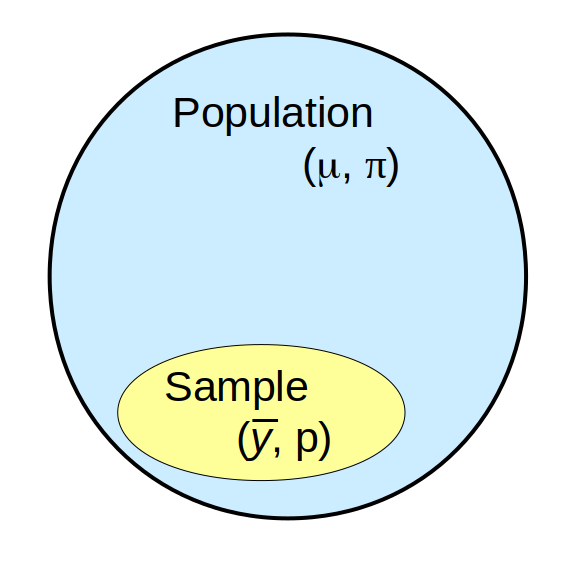
\includegraphics[scale=0.35]{MeansFig1.png}
	}
	
	
\end{frame}


\frame{\frametitle{Samples must be random} 
	
	\begin{itemize}
		\item 	The validity of inference will depend on the
		way that the sample was collected. If a sample was collected badly, no amount of
		statistical sophistication can rescue the study. \\ \ \\ 
		
		\item Samples should be \textbf{random}. That is, there should be no systematic set of
		characteristics that is related to the scientific question of interest that causes some
		people to be more likely to be sampled than others. The simplest type of randomization
		selects members from the population with equal probability (a uniform distribution). \\ \
		\\ 
		
		\pause
		
		\item 	\textbf{Do not cheat by}  
		\begin{itemize}
			\item 	Taking 5 people from the \emph{same} household to estimate
			
			\begin{itemize}
				\item proportion of Québécois who don't have a family doctor
				\item who saw a medical doctor last year
				\item average rent
			\end{itemize}  
			
			
			
			
			\item Sampling the depth of the ocean \emph{only around Montreal} to estimate \begin{itemize}
				\item proportion of  Earth's  surface  covered  by  water
			\end{itemize} 
			
		\end{itemize}
	\end{itemize}
}






\frame{\frametitle{Sampling Distributions} 
	
	\begin{defm}[Sampling Distribution]
		\begin{itemize}
			\setlength\itemsep{1.5em}
			\item The sampling distribution of a statistic is the distribution of values taken by the statistic in \textbf{all possible samples of the same size} from the same population.
			\item The standard deviation of a sampling distribution is called a \textbf{standard error}
		\end{itemize} 
	\end{defm}
	
	
	
}


\begin{frame}[fragile]{Sampling Distributions}
	
\begin{knitrout}\tiny
\definecolor{shadecolor}{rgb}{0.969, 0.969, 0.969}\color{fgcolor}\begin{figure}

{\centering 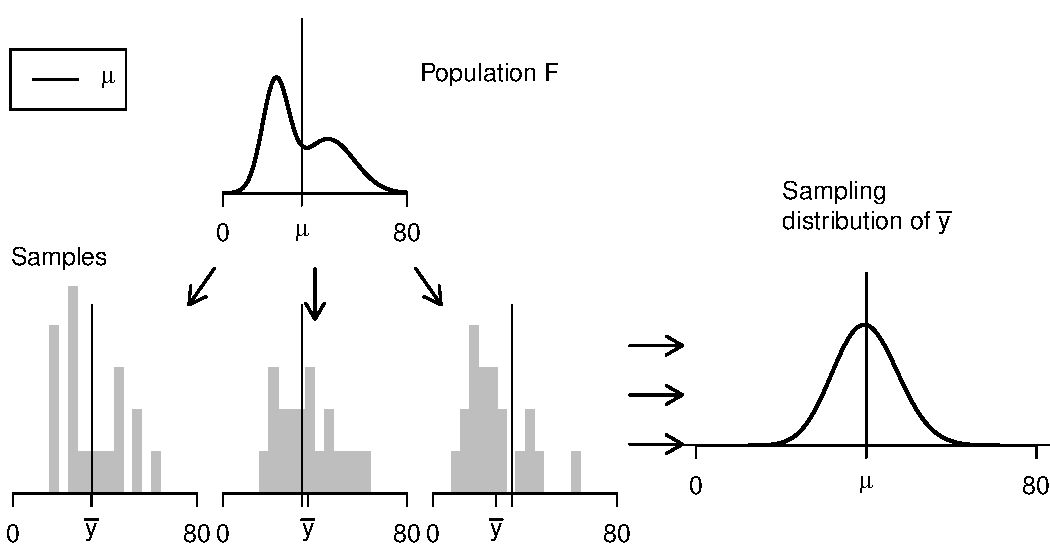
\includegraphics[width=\maxwidth]{figure/unnamed-chunk-7-1} 

}

\caption[Ideal world]{Ideal world. Sampling distributions are obtained by drawing repeated samples from the population, computing the statistic of interest for each, and collecting (an infinite number of) those statistics as the sampling distribution}\label{fig:unnamed-chunk-7}
\end{figure}


\end{knitrout}
	
\end{frame}


\frame{\frametitle{Why are sampling distributions important?} 
	
	\begin{itemize}
		\setlength\itemsep{2em} 
		\item They  tell  us  how  far  from  the  target  (true  value  of  the  parameter)  our  statistical  \emph{shot}  at  it  (i.e.  the  statistic  calculated  form  a  sample)  is  likely  to  be,  or, to  have  been.  \pause 
		
		\item Thus,  they  are  used  in  confidence  intervals  for  parameters. Specific  sampling  distributions  (based  on  a null value  for  the  parameter)  are also  used  in  statistical  tests  of  hypotheses.
		
	\end{itemize}	
	
	
}


\begin{frame}[fragile]{Sampling distribution: mean depth of the ocean}
	

	
\begin{knitrout}\tiny
\definecolor{shadecolor}{rgb}{0.969, 0.969, 0.969}\color{fgcolor}

{\centering 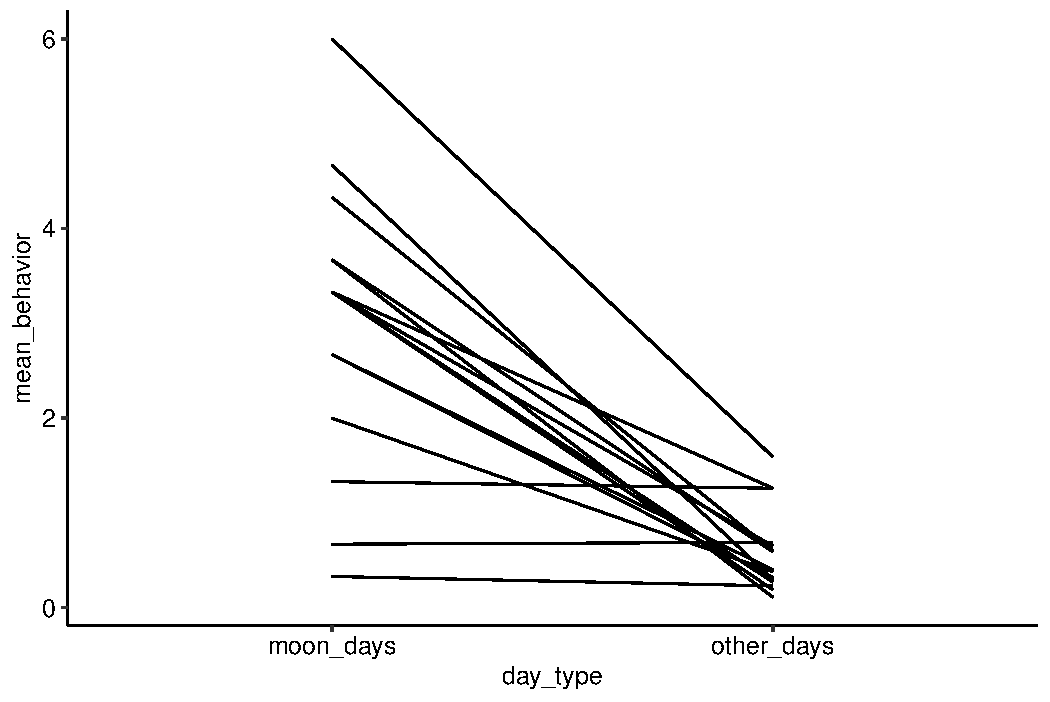
\includegraphics[width=\maxwidth]{figure/unnamed-chunk-9-1} 

}



\end{knitrout}
	
\end{frame}



\begin{frame}[fragile]{Sampling distribution: proportion covered by water}
	

	
	
\begin{knitrout}\tiny
\definecolor{shadecolor}{rgb}{0.969, 0.969, 0.969}\color{fgcolor}

{\centering 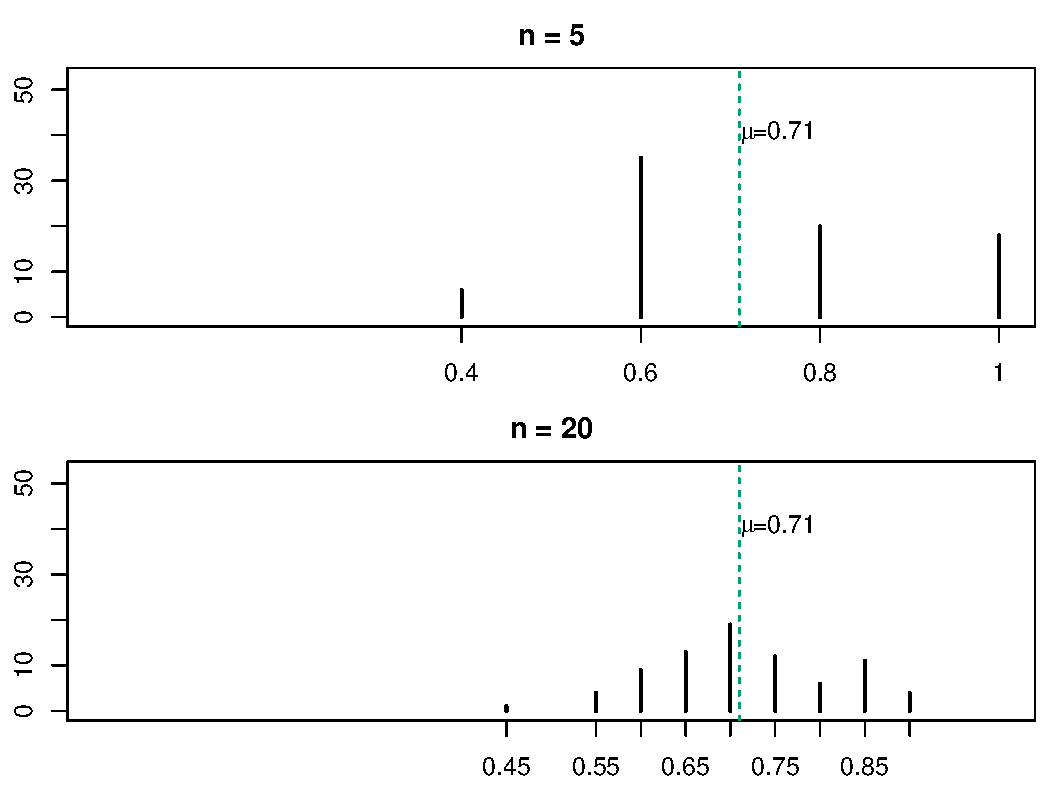
\includegraphics[width=\maxwidth]{figure/unnamed-chunk-11-1} 

}



\end{knitrout}
	
\end{frame}




\begin{frame}[fragile]{Normal Distribution: For probabilities we use $pnorm$}
	
	
\begin{knitrout}\tiny
\definecolor{shadecolor}{rgb}{0.969, 0.969, 0.969}\color{fgcolor}\begin{kframe}
\begin{alltt}
\hlstd{stats}\hlopt{::}\hlkwd{pnorm}\hlstd{(}\hlkwc{q} \hlstd{=} \hlnum{130}\hlstd{,} \hlkwc{mean} \hlstd{=} \hlnum{100}\hlstd{,} \hlkwc{sd} \hlstd{=} \hlnum{13}\hlstd{)}
\end{alltt}
\begin{verbatim}
## [1] 0.99
\end{verbatim}
\end{kframe}
\end{knitrout}
	
	
\begin{knitrout}\tiny
\definecolor{shadecolor}{rgb}{0.969, 0.969, 0.969}\color{fgcolor}\begin{kframe}
\begin{alltt}
\hlstd{mosaic}\hlopt{::}\hlkwd{xpnorm}\hlstd{(}\hlkwc{q} \hlstd{=} \hlnum{130}\hlstd{,} \hlkwc{mean} \hlstd{=} \hlnum{100}\hlstd{,} \hlkwc{sd} \hlstd{=} \hlnum{13}\hlstd{)}
\end{alltt}
\end{kframe}

{\centering 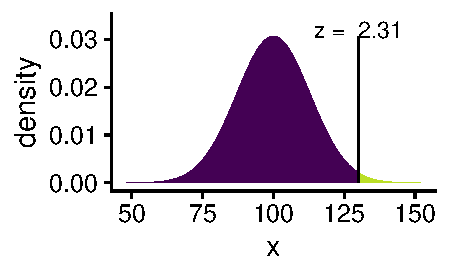
\includegraphics[width=0.6\linewidth]{figure/probs3-1} 

}


\begin{kframe}\begin{verbatim}
## [1] 0.99
\end{verbatim}
\end{kframe}
\end{knitrout}
	
	
	\begin{itemize}
		\item \texttt{pnorm} returns the integral from $-\infty$ to $q$ for a $\mathcal{N}(\mu, \sigma)$
		\item \texttt{pnorm} goes from \textit{quantiles} (think $Z$ scores) to probabilities
	\end{itemize}
	
\end{frame}



\begin{frame}[fragile]{Normal Distribution: For quantiles we use $qnorm$}
	
	
	
\begin{knitrout}\tiny
\definecolor{shadecolor}{rgb}{0.969, 0.969, 0.969}\color{fgcolor}\begin{kframe}
\begin{alltt}
\hlstd{stats}\hlopt{::}\hlkwd{qnorm}\hlstd{(}\hlkwc{p} \hlstd{=} \hlnum{0.0104}\hlstd{,} \hlkwc{mean} \hlstd{=} \hlnum{100}\hlstd{,} \hlkwc{sd} \hlstd{=} \hlnum{13}\hlstd{)}
\end{alltt}
\begin{verbatim}
## [1] 70
\end{verbatim}
\end{kframe}
\end{knitrout}
	
	
	
\begin{knitrout}\tiny
\definecolor{shadecolor}{rgb}{0.969, 0.969, 0.969}\color{fgcolor}\begin{kframe}
\begin{alltt}
\hlstd{mosaic}\hlopt{::}\hlkwd{xqnorm}\hlstd{(}\hlkwc{p} \hlstd{=} \hlnum{0.0104}\hlstd{,} \hlkwc{mean} \hlstd{=} \hlnum{100}\hlstd{,} \hlkwc{sd} \hlstd{=} \hlnum{13}\hlstd{)}
\end{alltt}
\end{kframe}

{\centering 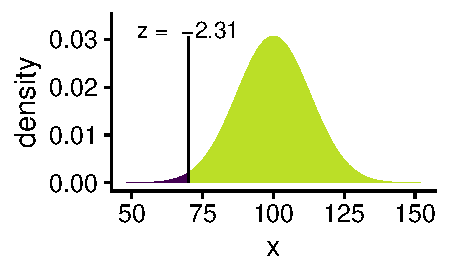
\includegraphics[width=0.6\linewidth]{figure/probs5-1} 

}


\begin{kframe}\begin{verbatim}
## [1] 70
\end{verbatim}
\end{kframe}
\end{knitrout}
	
	
	
	\small{
		\begin{itemize}
			\item \texttt{qnorm} answers the question: What is the Z-score of the $p$th percentile of the normal distribution?
			
			\item \texttt{qnorm} goes from \textit{probabilities} to quantiles 
		\end{itemize}
	}
\end{frame}

\begin{frame}[fragile]{Empirical Rule or 68-95-99.7\% Rule}
	
	\framedgraphic{6899rule.png}
	
\end{frame}



\begin{frame}[fragile]{Quadruple the work, half the benefit}
	
	\framedgraphiccaption{ROOToceanAll.png}{When the sample size increases from 4 to 16, the spread of the sampling distribution for the mean is reduced by a half, i.e., the range is cut in half. This is known as the curse of the $\sqrt{n}$}
\end{frame}


\frame{\frametitle{The Central Limit Theorem (CLT)} 
	
	\begin{itemize}
		\item The sampling distribution of $\bar{y}$ is, for a large enough $n$, close to Gaussian in shape no matter what the shape of the distribution of individual $Y$ values. 
		\item This phenomenon is referred to as the CENTRAL LIMIT THEOREM 
		\item The CLT applied also to a \underline{sample proportion}, \underline{slope}, \underline{correlation}, or any other statistic created by \underline{aggregation of individual observations}
	\end{itemize}
	
	\begin{thm}[Central Limit Theorem]
		\begin{center}
			if $Y \sim ???(\mu_Y, \sigma_Y)$, then \\ \ \\
			$\bar{y} \sim \mathcal{N}(\mu_Y, \sigma_Y / \sqrt{n})$
		\end{center}
	\end{thm}
	
	\vspace{1.25cm}
	%pause
}

\begin{frame}{Confidence Interval}
	
	\begin{defm}[Confidence Interval]
		A level $C$ confidence interval for a parameter has two parts:
		\begin{enumerate}
			\item An interval calculated from the data, \underline{usually} of the form $$\textrm{estimate} \pm \textrm{margin of error}$$ where the estimate is a sample statistic and the margin of error represents the accuracy of our guess for the parameter.
			\item A confidence level $C$, which gives the probability that the interval will capture the true parameter value in \textit{different possible samples}. That is, the confidence level is the success rate for the method
		\end{enumerate}
	\end{defm}
	
	%\framedgraphic{6899rule.png}
	
\end{frame}

\frame{\frametitle{Confidence Interval: A simulation study}
	
	\vspace*{-0.1in}
	
	\begin{figure}
		\begin{center}
			\epsfig{figure=CIplots.eps,width=3.2in,height=2.7in}
			\caption{\small{True parameter value is 2 (red line). Each horizontal black line represents a 95\% CI from a sample and contains the true parameter value. The blue CIs do not contain the true parameter value. 95\% of all samples give an interval that contains the population parameter.}}
		\end{center}
	\end{figure}
}


\begin{frame}{Interpreting a frequentist confidence interval}
	\begin{itemize}
		\setlength\itemsep{1em}
		\item The confidence level is the success rate of the method that produces the interval. \pause
		\item We don't know whether the 95\% confidence interval from a \underline{particular
			sample} is one of the 95\% that capture $\theta$ (the unknown population parameter), or one of the unlucky 5\% that miss. \pause
		\item To say that we are \underline{95\% confident} that the unknown value of $\theta$
		lies between $U$ and $L$ is shorthand for ``We got these numbers using a
		method that gives correct results 95\% of the time.''
	\end{itemize}
\end{frame}

\begin{frame}[fragile]{68\% Confidence interval using \texttt{qnorm}}
	

	
	
	\vspace*{-0.09in}
	
	\Wider[2em]{
\begin{knitrout}\tiny
\definecolor{shadecolor}{rgb}{0.969, 0.969, 0.969}\color{fgcolor}\begin{figure}

{\centering 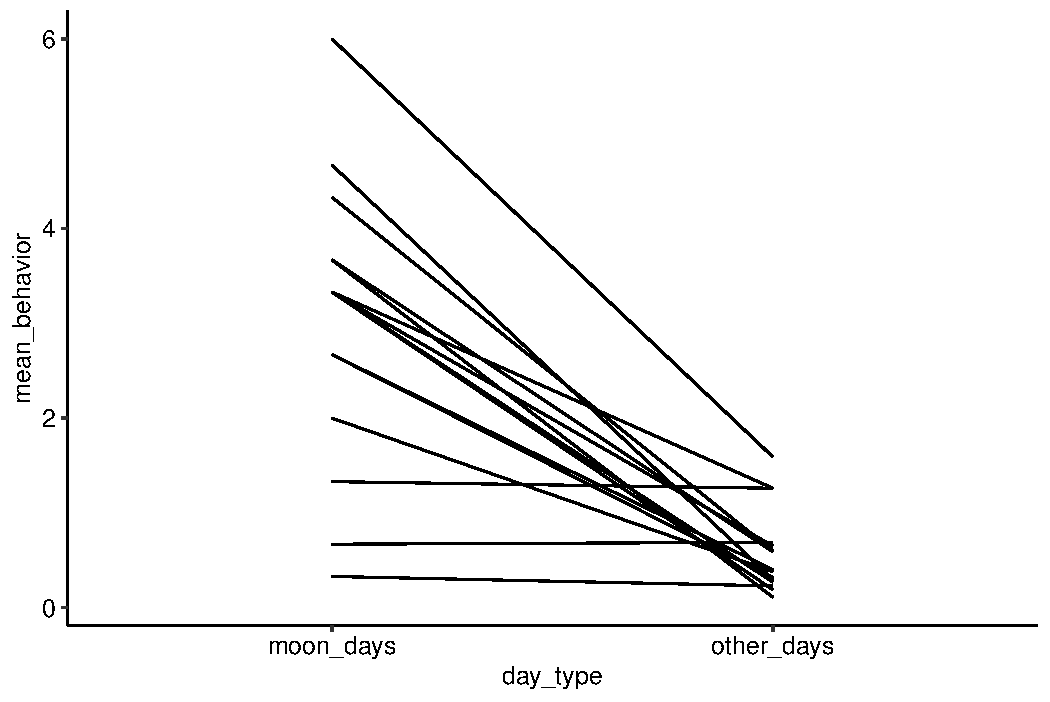
\includegraphics[width=\maxwidth]{figure/unnamed-chunk-13-1} 

}

\caption{68\% Confidence interval calculated using  \mbox{\texttt{qnorm(p = c(0.16,0.84), mean = 37, sd = 4.2)}}}\label{fig:unnamed-chunk-13}
\end{figure}


\end{knitrout}
		
	}
\end{frame}



\begin{frame}[fragile]{95\% Confidence interval using \texttt{qnorm}}
	
	\vspace*{-0.09in}
	
	
	\Wider[2em]{
\begin{knitrout}\tiny
\definecolor{shadecolor}{rgb}{0.969, 0.969, 0.969}\color{fgcolor}\begin{figure}

{\centering 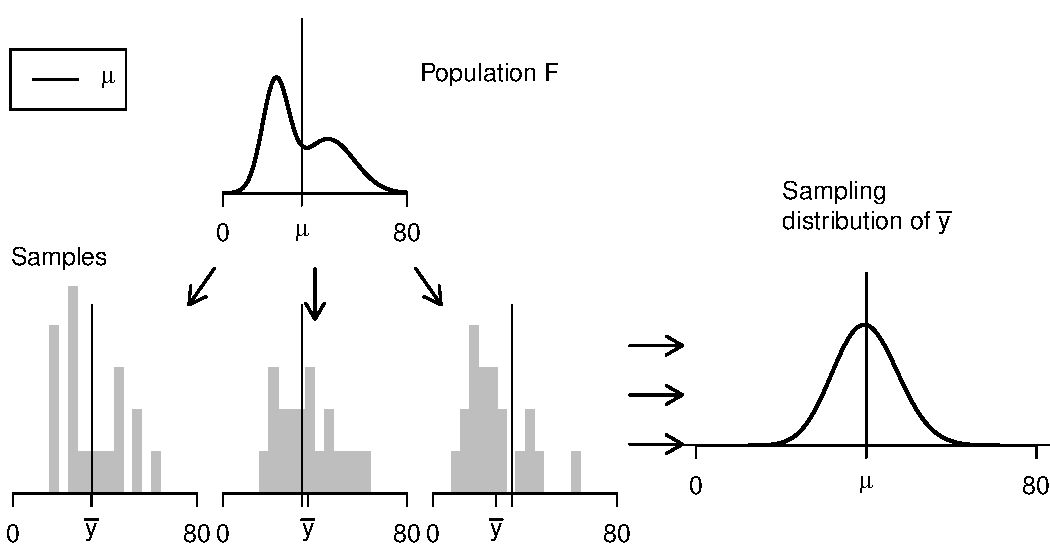
\includegraphics[width=\maxwidth]{figure/unnamed-chunk-14-1} 

}

\caption{95\% Confidence interval calculated using  \mbox{\texttt{qnorm(p = c(0.025,0.975), mean = 37, sd = 4.2)}}}\label{fig:unnamed-chunk-14}
\end{figure}


\end{knitrout}
		
	}
	
\end{frame}

\frame{\frametitle{Example: Inference for a single population mean} So what
	does the CI allow us to learn about $\mu$??
	\begin{itemize}
		\setlength\itemsep{2em}
		\item It tells us that if we repeated this procedure again and again
		(collecting a sample mean, and constructing a 95\% CI), 95\% of the
		time, the CI would \textit{cover} $\mu$. \pause 
		\item That is, with 95\% probability, the \textit{procedure}
		will include the true value of $\mu$. Note that we are making \underline{a probability statement about the CI}, not about the parameter. \pause
		\item Unfortunately, \textcolor{blue}{we do not know whether the true value of $\mu$ is
			contained in the CI in the particular experiment that we have
			performed.}
	\end{itemize}
}



\section{Bootstrap}

\begin{frame}{Motivation for the Bootstrap}
	\begin{itemize}
		\setlength\itemsep{2em}
		\item The $\pm$ and \texttt{qnorm} methods to calculate a CI both require the CLT
	\end{itemize}
	
	\pause
	
	\vspace*{0.2in}
	
	\Large \textcolor{myblue}{Q: What happens if the CLT hasn't `kicked in`? Or you don't believe the CLT?} \\ \ \\
	\pause 
	\Large \textcolor{myblue}{Q: What happens if there is no formula available to calculate a CI?} \\ \ \\
	\pause 
	\Large \textcolor{red}{A: Bootstrap} \\ \ \\
\end{frame}



\begin{frame}[fragile]{Ideal world: known sampling distribution}
	
\begin{knitrout}\tiny
\definecolor{shadecolor}{rgb}{0.969, 0.969, 0.969}\color{fgcolor}\begin{figure}

{\centering 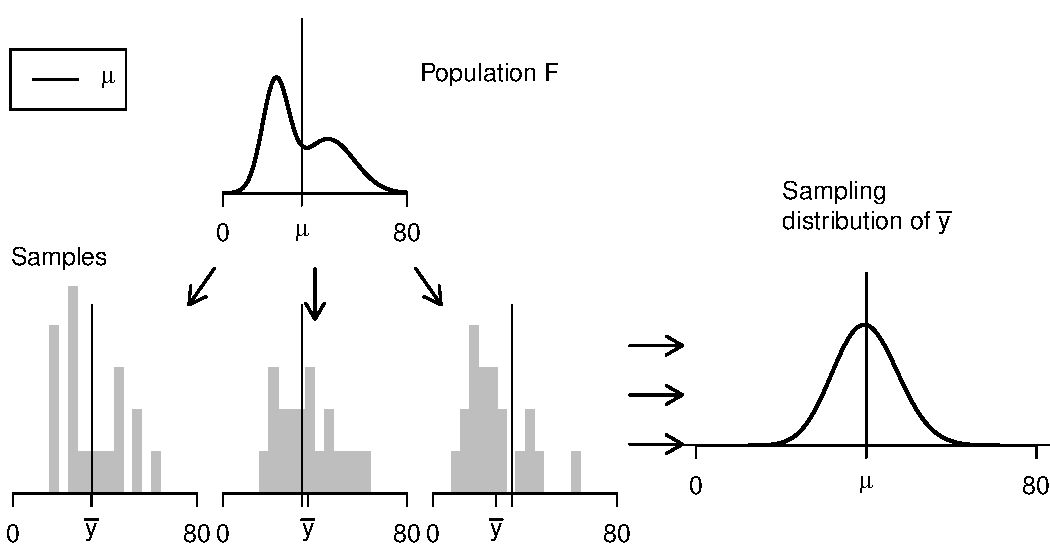
\includegraphics[width=\maxwidth]{figure/unnamed-chunk-15-1} 

}

\caption{\scriptsize{Ideal world. Sampling distributions are obtained by drawing repeated samples from the population, computing the statistic of interest for each, and collecting (an infinite number of) those statistics as the sampling distribution}}\label{fig:unnamed-chunk-15}
\end{figure}


\end{knitrout}
	
\end{frame}



\begin{frame}[fragile]{Reality: use the bootstrap distribution instead}
	
	

	
	\framedgraphiccaption{boot_diag.pdf}{\scriptsize{Bootstrap world. The bootstrap distribution is obtained by drawing repeated samples from an estimate of the population, computing the statistic of interest for each, and collecting those statistics. The distribution is centered at the observed statistic ($\bar{y}$), not the parameter ($\mu$).}}
	
\end{frame}


\begin{frame}[fragile]{Main idea: simulate your own sampling distribution}
	

	
\begin{knitrout}\tiny
\definecolor{shadecolor}{rgb}{0.969, 0.969, 0.969}\color{fgcolor}\begin{kframe}
\begin{alltt}
\hlstd{R} \hlkwb{<-} \hlkwd{replicate}\hlstd{(B, \{}
\hlstd{dplyr}\hlopt{::}\hlkwd{sample_n}\hlstd{(depths.n.20,} \hlkwc{size} \hlstd{= N,} \hlkwc{replace} \hlstd{=} \hlnum{TRUE}\hlstd{)} \hlopt
\hlstd{dplyr}\hlopt{::}\hlkwd{summarize}\hlstd{(}\hlkwc{r} \hlstd{=} \hlkwd{mean}\hlstd{(alt))} \hlopt
\hlstd{dplyr}\hlopt{::}\hlkwd{pull}\hlstd{(r)}
\hlstd{\})}
\hlstd{CI_95} \hlkwb{<-} \hlkwd{quantile}\hlstd{(R,} \hlkwc{probs} \hlstd{=} \hlkwd{c}\hlstd{(}\hlnum{0.025}\hlstd{,} \hlnum{0.975}\hlstd{))}
\end{alltt}
\end{kframe}

{\centering 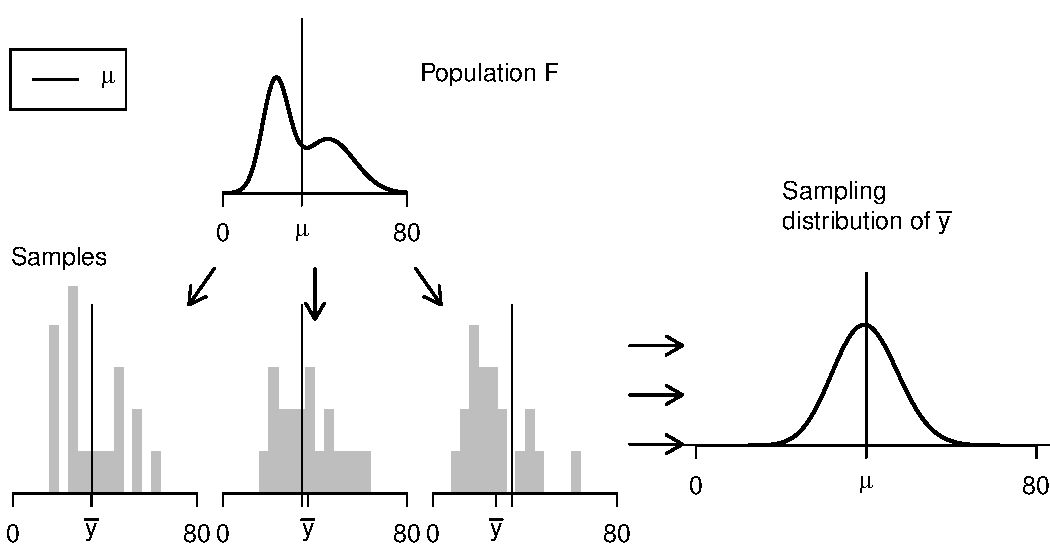
\includegraphics[width=\maxwidth]{figure/unnamed-chunk-18-1} 

}



\end{knitrout}
	
\end{frame}

\begin{frame}{Bootstrap can be used for other statistics (e.g. $R^2$)}
	\centering
	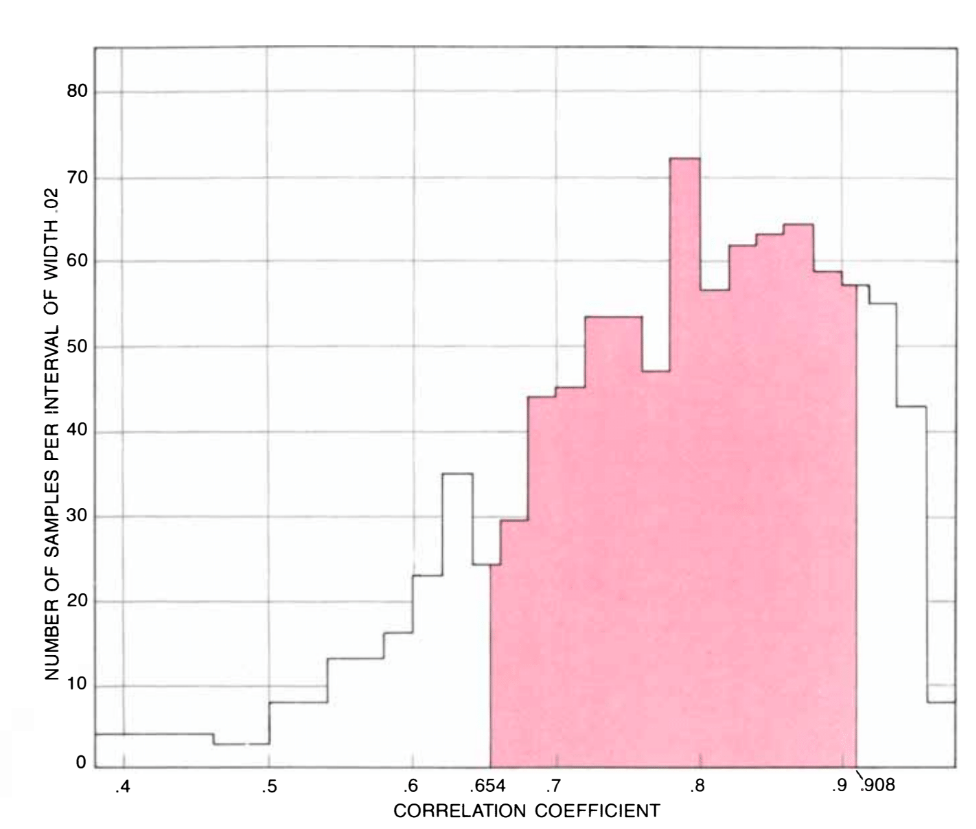
\includegraphics[scale=0.29]{bootcorr.png}
	
	\vspace{0.1in}
	
	\tiny \href{https://www.dropbox.com/s/cxiq70zxxtyxlb5/EfronDiaconisBootstrap.pdf?dl=0}{source: Bootstrap article in Scientific American}
\end{frame}


\section{One sample mean}


\begin{frame}{$\sigma$ known vs. unknown}
	\begin{center}
		\begin{tabular}{|l|c|c|} \hline
			$\sigma$& known & unknown \\ \hline Data & $\{y_1,y_2,...,y_n\}$ &
			$\{y_1,y_2,...,y_n\}$\\
			& & \\
			Pop'n param & $\mu$ & $\mu$\\
			& & \\
			Estimator & $\overline{y} = \frac{1}{n}\sum_{i=1}^n y_i$ & $\overline{y} = \frac{1}{n}\sum_{i=1}^n y_i$ \\
			& & \\
			SD & $\sigma$ & $s = \sqrt{\frac{\sum_{i=1}^n(y_i-\overline{y})^2}{n-1}}$ \\
			& & \\
			SEM & $\sigma/\sqrt{n}$ & $s / \sqrt{n}$ \\
			& & \\
			$(1-\alpha)100$\% CI & $\overline{y} \pm z^\star_{1-\alpha/2}$(SEM) & $\overline{y} \pm t^\star_{1-\alpha/2, (n-1)}$(SEM) \\
			& & \\
			test statistic & $\frac{\overline{y}-\mu_0}{\textrm{SEM}}\sim \mathcal{N}(0,1)$ &
			$\frac{\overline{y}-\mu_0}{\textrm{SEM}}\sim t_{(n-1)}$ \\
			\hline
		\end{tabular}
	\end{center}
\end{frame}


\begin{frame}{Assumptions}
	\Wider[3em]{
		\begin{center}
			\begin{tabular}{|l|c|c|c|} \hline
				& $z$ & $t$ & Bootstrap \\ 
				\hline 
				SRS & \cmark &\cmark &	\cmark\\
				& & & \\
				Normal population & \cmark$^\star$ & \cmark$^\star$ &  \xmark\\
				& & &\\
				needs CLT &  \cmark$^\star$ & \cmark$^\star$ &  \xmark\\
				& & &\\
				$\sigma$ known  & \cmark & \xmark & \xmark\\
				& & &\\
				Sampling dist. center at & $\mu$ & $\mu$ & $\bar{y}$\\
				& & &\\
				SD & $\sigma$ & $s$ & $s$ \\
				& & &\\
				SEM & $\sigma/\sqrt{n}$ & $s / \sqrt{n}$ & SD(bootstrap statistics) \\
				\hline
			\end{tabular}
			
			\footnotetext[1]{*If population is Normal then CLT is not needed. If population is not Normal then CLT is needed.}
		\end{center}
	}
\end{frame}

\section{One sample proportion}

\begin{frame}
	\begin{itemize}
		\item Binomial calculations
		\item Nomogram, Clopper-Pearson CI
		\item Normal approximation
	\end{itemize}
\end{frame}


\section{p-values}

\begin{frame}
	\frametitle{$p$-values and statistical tests}
	
	
	%\vspace{18pt}
	\begin{defm}[$p$-value]
		A \textbf{probability concerning the observed data}, calculated under a \textbf{Null Hypothesis} assumption, i.e., assuming that the only factor operating is sampling or measurement variation. 
	\end{defm}
	
	\begin{itemize} 
		\item[\underline{Use}] To assess the evidence provided by the sample data
		in relation to a pre-specified claim or `hypothesis' concerning some parameter(s) or data-generating process. 
		\item[\underline{Basis}] As with a confidence interval, it makes use of the concept of a \textit{distribution}. 
		\item[\underline{Caution}] A $p$-value is NOT the probability that the null `hypothesis' is true
	\end{itemize}
\end{frame}


\begin{frame}
	\frametitle{More about the $p$-value}
	\small
	%\begin{footnotesize}
	\begin{itemize}
		\setlength\itemsep{.3em}
		\item The $p$-value is a \textbf{probability concerning data}, \textbf{conditional on the Null Hypothesis being true}. \pause
		\item \textbf{It is not the probability that Null Hypothesis is true}, \textit{conditional on the data.} \pause
		%\item Very few MDs mix up complement of specificity (i.e. probability of a `positive'  test result when in fact patient does not have disease in question) with positive predictive value (i.e. probability that a patient who has had a `positive'  test result does  have disease in question).
		\begin{align*}
			p_{value} & = P(\textrm{this or more extreme data}| H_0) \\
			& \neq P(H_0|\textrm{this or more extreme data}).
		\end{align*}
		
		\pause 
		\item Statistical tests are often coded as statistically significant or not according to whether results are extreme or not with respect to a reference (null)  distribution.  But a test result  is just one piece of data, and needs to be considered \textit{along with  rest of evidence} before coming to a `conclusion.' \item \textbf{Likewise with statistical `tests': the $p$-value is just one more piece of \textit{evidence}, hardly enough to `conclude' anything}. 
		%\item The probability that the DNA from the blood  of a randomly selected (innocent) person would match that from blood on crime-scene glove was 
		%$p=10^{-17}$. \textit{Do not equate this} Prob[data $|$ innocent] \textit{with its transpose}:
		%writing ``data'' as shorthand for ``this or more extreme data'', we need to be aware that 
		%$$p_{value} = Prob[ \ data \  | \  H_0 ] \neq Prob[ \ H_0 \  |  \ data ].$$
	\end{itemize}
	%\end{footnotesize}
\end{frame}

\begin{frame}
	\frametitle{Close relationship between $p$-value and CI}
	\begin{center}
		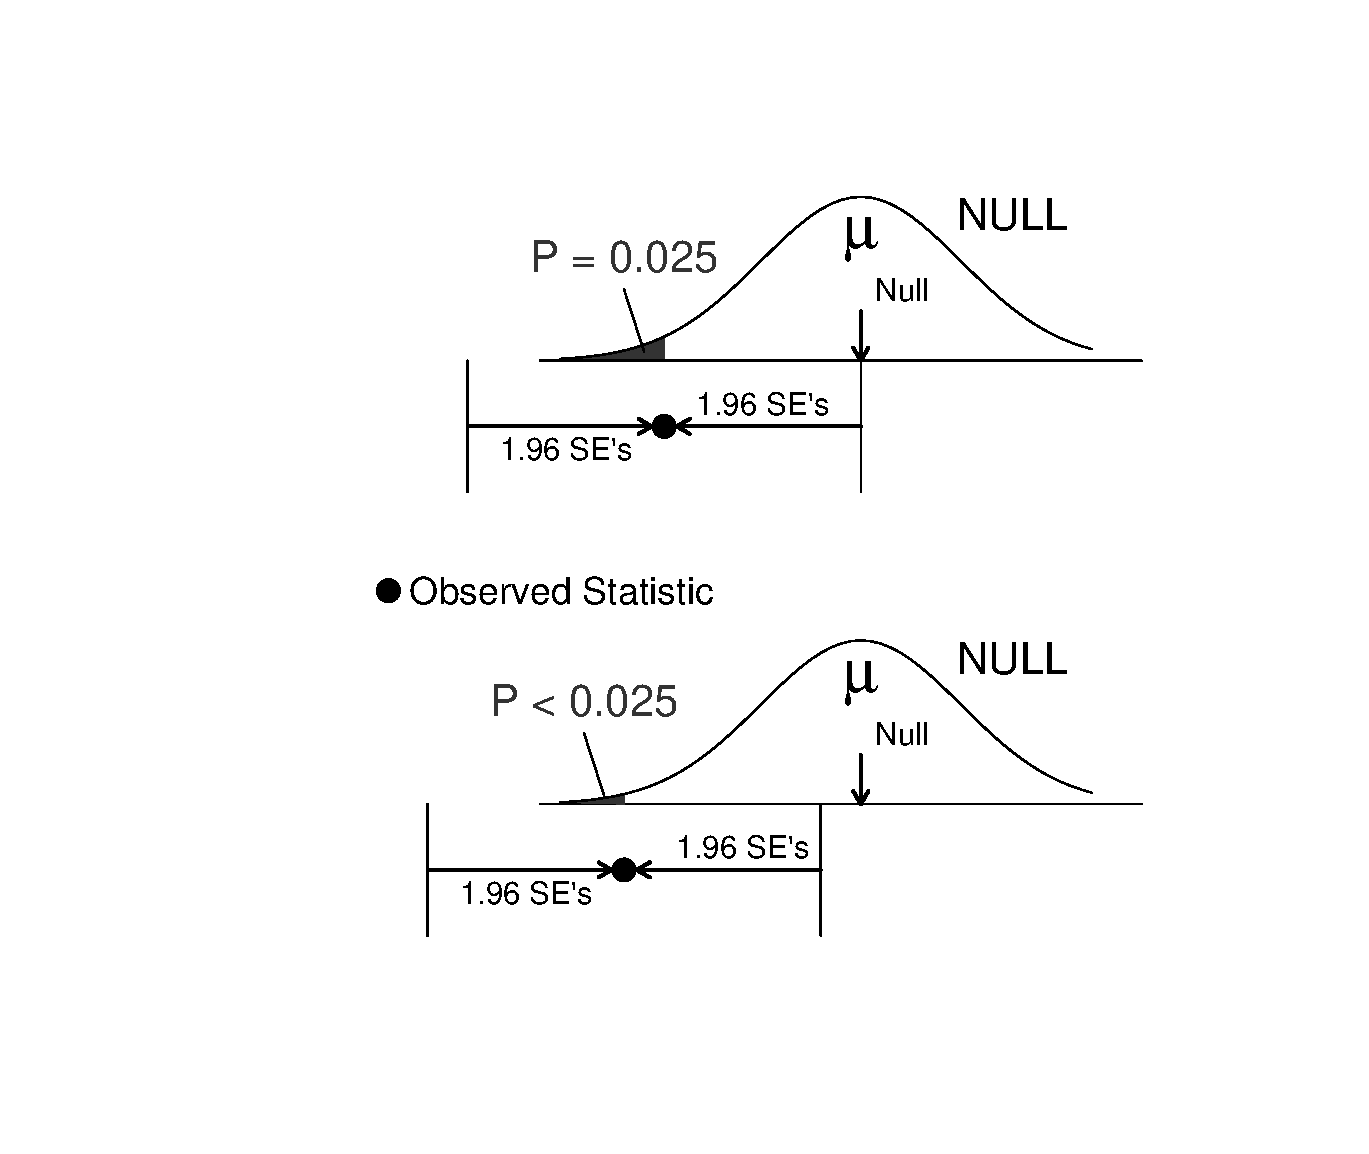
\includegraphics[width=1.65in]{P-CI.pdf}
	\end{center} 
	\begin{footnotesize}
		\begin{itemize}
			\item
			(Upper graph) If upper limit of 95\% CI\textit{ just touches} null value, then
			the 2 sided $p$-value is 0.05 (or 1 sided $p$-value is 0.025). 
			\item
			(Lower graph) If upper limit \textit{excludes} null value, then
			the 2 sided $p$-value is less than 0.05 (or 1 sided $p$-value is less than 0.025). 
			\item
			(Graph not shown) If  CI \textit{includes} null value, then the 2-sided $p$-value is greater than (the conventional) 0.05, and thus observed statistic is ``not statistically significantly different'' from hypothesized null value. 
		\end{itemize}
	\end{footnotesize}
\end{frame}


\section{Power and sample size}

\begin{frame}[fragile]{Power = $1 - \beta$}
	
	\vspace*{-0.2in}
	
	\begin{defm}[Power = $1-\beta$]
		The probability that a fixed level $\alpha$ significance test will reject $H_0$ when a particular alternative value of the parameter is true is called the \textbf{power} of the test to detect the alternative. 
	\end{defm}
	
	
	\vspace*{-0.08in}
	
	\centering
	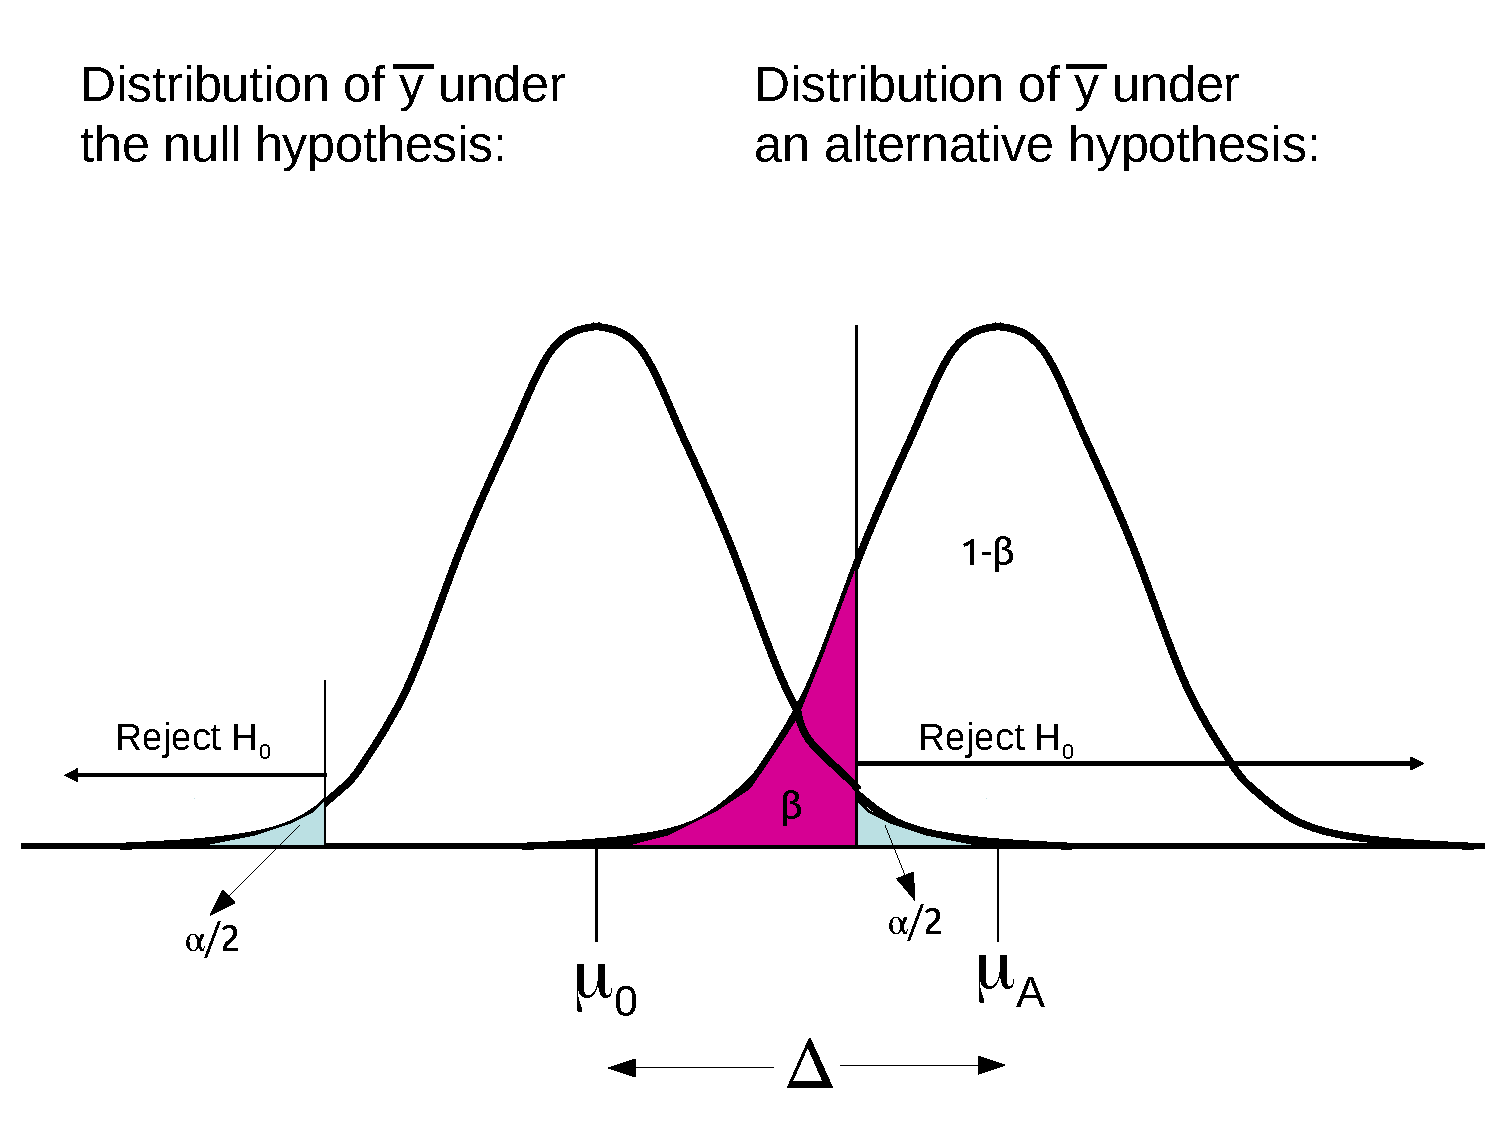
\includegraphics[scale=0.31]{HypTest3-3.pdf}
	
	
\end{frame}

\begin{frame}{Power and Sample Size: 3 questions}
	
	\begin{enumerate}
		\setlength\itemsep{1em}
		\item How much water a supplier could add to the milk before they have a 10\% , 50\%, 80\%
		chance of getting caught, i.e., of the buyer detecting the cheating ? \pause
		\item Assume a 99:1 mix of milk and water. What are the chances of detecting cheating if the buyer uses samples $n$=10, 15 or 20 rather than just 5 measurements? \pause
		\item At what $n$ does the chance of detecting cheating reach 80\%? (\textit{a commonly used, but arbitrary, criterion used in sample-size planning by investigators seeking funding for their proposed research})
	\end{enumerate}
	
\end{frame}


\begin{frame}[fragile]{If the supplier added 1\% water to the milk}
\begin{knitrout}\tiny
\definecolor{shadecolor}{rgb}{0.969, 0.969, 0.969}\color{fgcolor}

{\centering 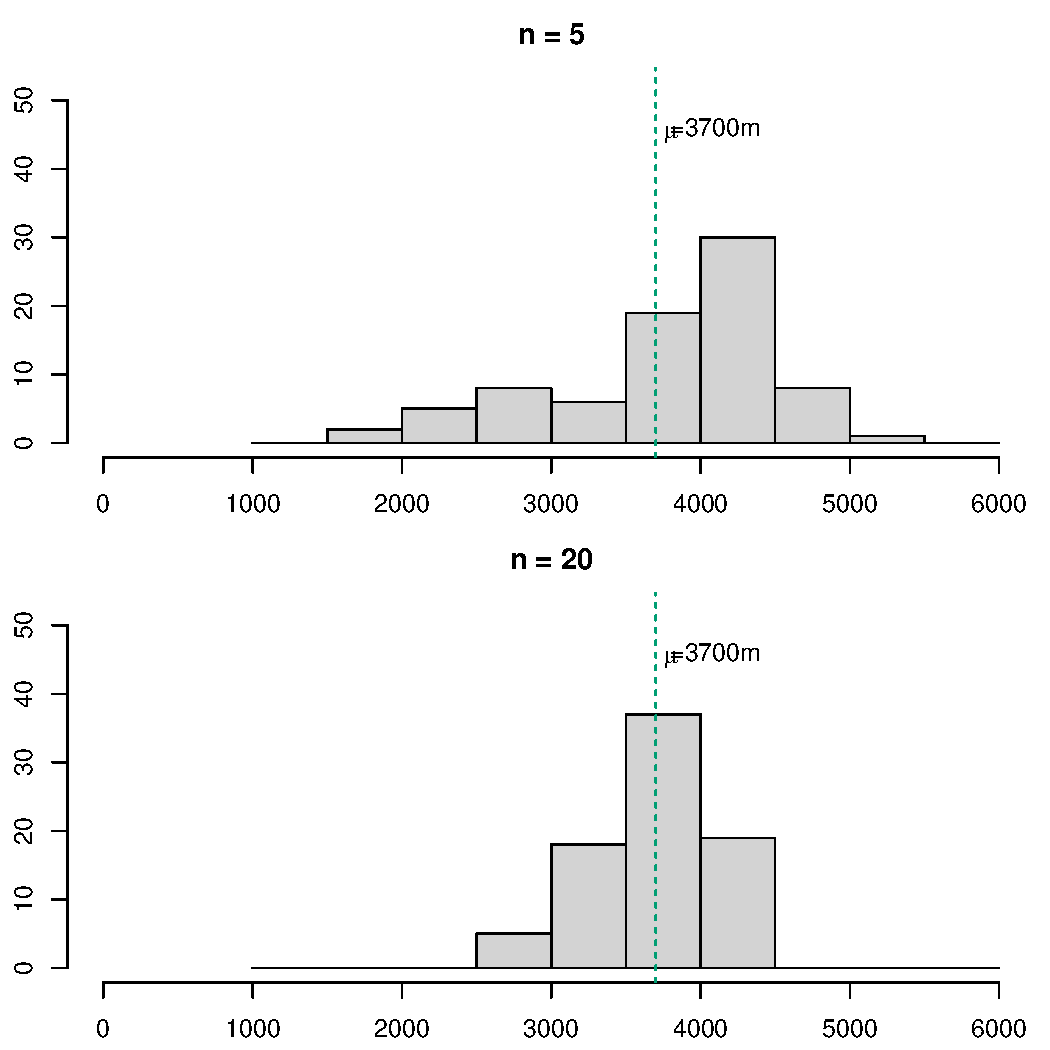
\includegraphics[width=\maxwidth]{figure/unnamed-chunk-19-1} 

}



\end{knitrout}
\end{frame}



\begin{frame}
	
	\begin{center}
		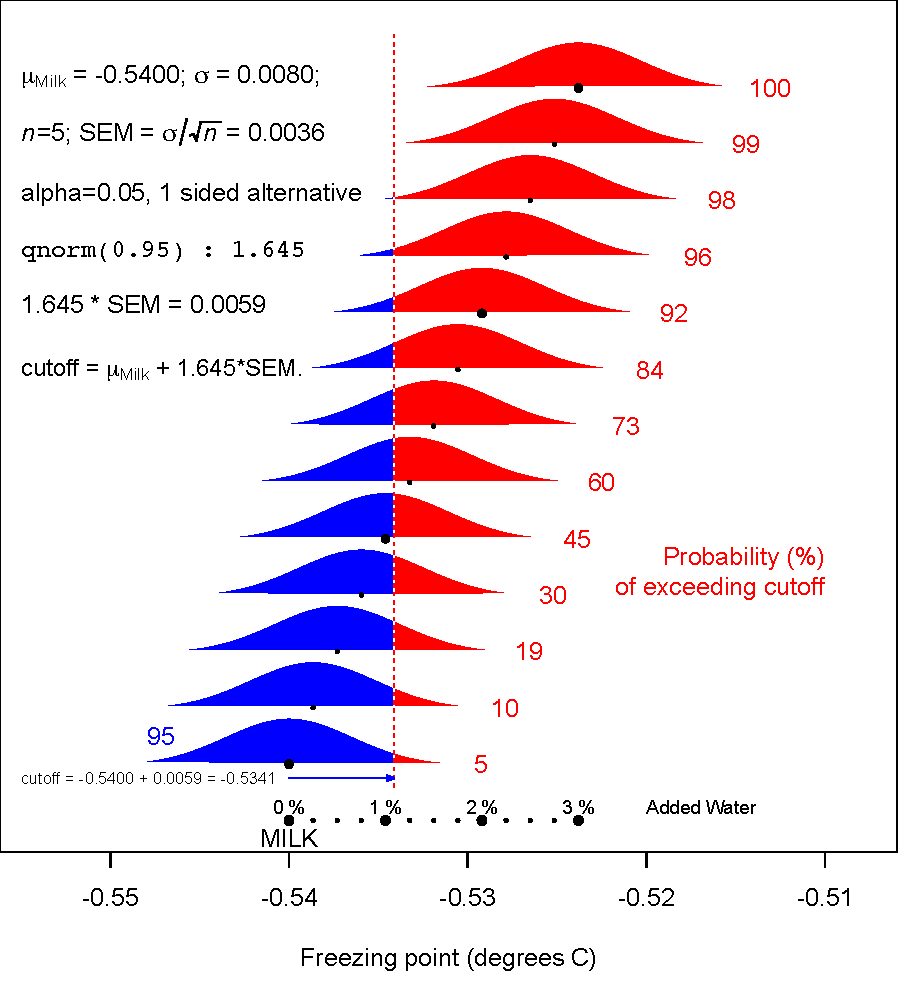
\includegraphics[scale=0.45]{ProbDetectingWaterInMilk.pdf} 
	\end{center}
	
	\vspace*{-0.18in}
	
	{ \footnotesize
		The probabilities in red were calculated using the formula:
		\texttt{stats::pnorm(cutoff, mean = mu.mixture, sd = SEM, lower.tail=FALSE)}
	}
\end{frame}


\begin{frame}
	\begin{center}
		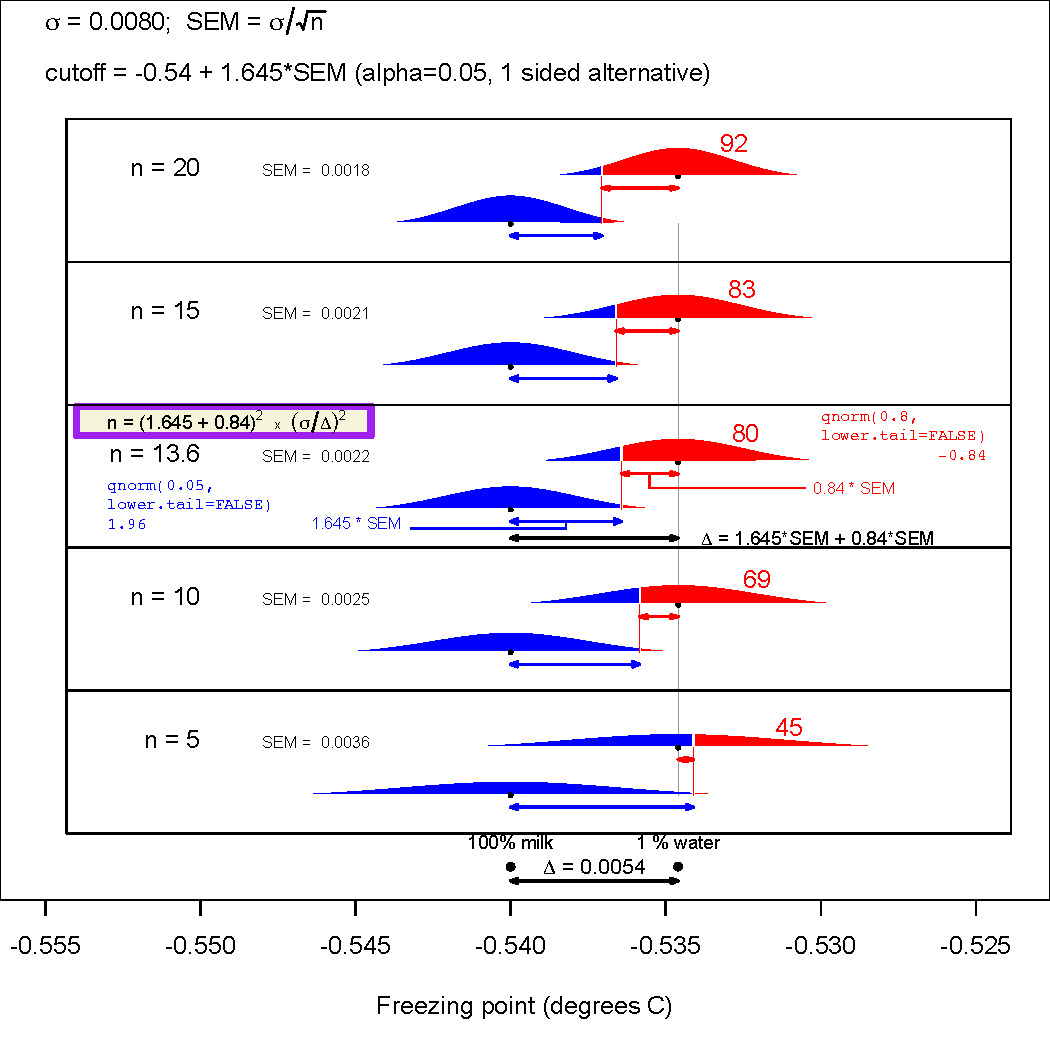
\includegraphics[scale=0.5]{SampleSize1pctWaterAdded.pdf} 
	\end{center}
\end{frame}

\begin{frame}[fragile]{The balancing formula}
\begin{knitrout}\tiny
\definecolor{shadecolor}{rgb}{0.969, 0.969, 0.969}\color{fgcolor}

{\centering 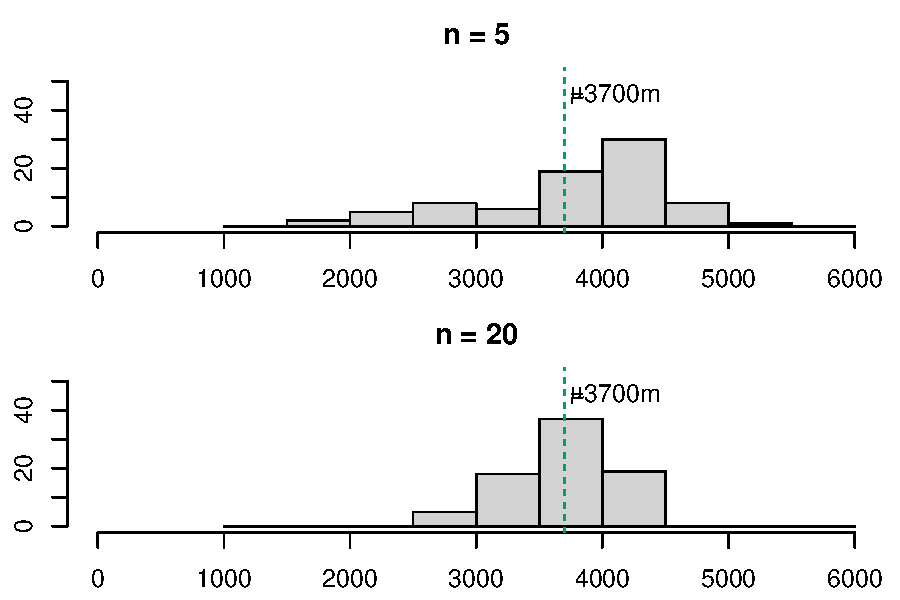
\includegraphics[width=\maxwidth]{figure/unnamed-chunk-20-1} 

}



\end{knitrout}
\end{frame}


\begin{frame}{What sample size needed?}
	
	\begin{itemize}
		\setlength\itemsep{1em}
		\item The `balancing formula', in SEM terms, is simply the $n$ where
		$$ 1.645 \times SEM + 0.84 \times SEM = \Delta.$$
		Replacing each of the  SEMs (assumed equal, because we assumed the variability
		is approx. the same under both scenarios) by $\sigma/\sqrt{n}$,  i.e.,
		
		$$ 1.645 \times \sigma/\sqrt{n} + 0.84 \times \sigma/\sqrt{n} = \Delta.$$
		
		and solving for $n$, one gets
		
		$$  n = (1.645 + 0.84)^2  \times \bigg\{ \frac{\sigma}{\Delta} \bigg\}^2 = 
		(1.645 + 0.84)^2  \times \bigg\{ \frac{Noise}{Signal} \bigg\}^2 .$$
	\end{itemize}
	
\end{frame}

\begin{frame}{What sample size needed? General Formula}
	
	\begin{itemize}
		\setlength\itemsep{2em}
		\item Two sided alternative:
		$$\Delta = z_{1-\alpha/2} \times SEM + z_{1-\beta} \times SEM$$
		
		\item One sided alternative:
		$$\Delta = z_{1-\alpha} \times SEM + z_{1-\beta} \times SEM$$
	\end{itemize}
	
\end{frame}



\begin{frame}[fragile]{Session Info}
	\tiny
	
\begin{knitrout}\tiny
\definecolor{shadecolor}{rgb}{0.969, 0.969, 0.969}\color{fgcolor}\begin{kframe}
\begin{verbatim}
R version 4.0.2 (2020-06-22)
Platform: x86_64-pc-linux-gnu (64-bit)
Running under: Pop!_OS 20.04 LTS

Matrix products: default
BLAS:   /usr/lib/x86_64-linux-gnu/openblas-pthread/libblas.so.3
LAPACK: /usr/lib/x86_64-linux-gnu/openblas-pthread/liblapack.so.3

attached base packages:
[1] tools     stats     graphics  grDevices utils     datasets  methods  
[8] base     

other attached packages:
 [1] latex2exp_0.4.0    RColorBrewer_1.1-2 colorspace_1.4-1   oibiostat_0.2.0   
 [5] NCStats_0.4.7      FSA_0.8.30         forcats_0.5.0      stringr_1.4.0     
 [9] dplyr_1.0.2        purrr_0.3.4        readr_1.3.1        tidyr_1.1.2       
[13] tibble_3.0.3       ggplot2_3.3.2      tidyverse_1.3.0    knitr_1.29        

loaded via a namespace (and not attached):
  [1] minqa_1.2.4        TH.data_1.0-10     ellipsis_0.3.1    
  [4] rio_0.5.16         leaflet_2.0.3      sjlabelled_1.1.7  
  [7] snakecase_0.11.0   estimability_1.3   ggstance_0.3.4    
 [10] parameters_0.8.6   ggdendro_0.1.22    fs_1.5.0          
 [13] rstudioapi_0.11    farver_2.0.3       ggrepel_0.8.2     
 [16] fansi_0.4.1        mvtnorm_1.1-1      lubridate_1.7.9   
 [19] xml2_1.3.2         mosaic_1.7.0       codetools_0.2-16  
 [22] splines_4.0.2      sjmisc_2.8.5       polyclip_1.10-0   
 [25] jsonlite_1.7.1     nloptr_1.2.2.2     ggeffects_0.16.0  
 [28] broom_0.7.0        dbplyr_1.4.4       ggforce_0.3.2     
 [31] effectsize_0.3.3   compiler_4.0.2     httr_1.4.2        
 [34] sjstats_0.18.0     emmeans_1.5.1      backports_1.1.9   
 [37] assertthat_0.2.1   Matrix_1.2-18      cli_2.0.2         
 [40] tweenr_1.0.1       htmltools_0.5.0    coda_0.19-4       
 [43] gtable_0.3.0       glue_1.4.2         Rcpp_1.0.5        
 [46] carData_3.0-4      cellranger_1.1.0   vctrs_0.3.4       
 [49] sjPlot_2.8.5       nlme_3.1-149       crosstalk_1.1.0.1 
 [52] insight_0.9.6      xfun_0.17          lme4_1.1-23       
 [55] openxlsx_4.1.5     rvest_0.3.6        lifecycle_0.2.0   
 [58] mosaicCore_0.8.0   pacman_0.5.1       statmod_1.4.34    
 [61] MASS_7.3-53        zoo_1.8-8          scales_1.1.1      
 [64] hms_0.5.3          sandwich_2.5-1     curl_4.3          
 [67] mosaicData_0.20.1  gridExtra_2.3      TeachingDemos_2.12
 [70] stringi_1.5.3      highr_0.8          bayestestR_0.7.2  
 [73] boot_1.3-25        zip_2.1.1          rlang_0.4.7       
 [76] pkgconfig_2.0.3    evaluate_0.14      lattice_0.20-41   
 [79] htmlwidgets_1.5.1  labeling_0.3       tidyselect_1.1.0  
 [82] ggformula_0.9.4    plyr_1.8.6         magrittr_1.5      
 [85] R6_2.4.1           generics_0.0.2     multcomp_1.4-13   
 [88] DBI_1.1.0          pillar_1.4.6       haven_2.3.1       
 [91] foreign_0.8-79     withr_2.2.0        survival_3.2-3    
 [94] abind_1.4-5        performance_0.5.0  modelr_0.1.8      
 [97] crayon_1.3.4       car_3.0-9          utf8_1.1.4        
[100] grid_4.0.2         readxl_1.3.1       data.table_1.13.0 
[103] blob_1.2.1         reprex_0.3.0       digest_0.6.25     
[106] xtable_1.8-4       munsell_0.5.0      viridisLite_0.3.0 
\end{verbatim}
\end{kframe}
\end{knitrout}
	
\end{frame}

\end{document}
